    \section{Bulgular ve Senaryo Analizi}

    Senaryolardaki çizge yapısı \autoref{sec:kümeler-ve-parametreler}'de tanımlandığı gibidir. Analizlerde aksi belirtilmedikçe buradaki çizge yapılandırması kullanılacaktır.
    
    \subsection{Zıt Yön Çatışması}
    
    Bu senaryoda yazılan programın dinamik başlangıç özelliğinden yararlanarak araçların olası zıt yönde karşı karşıya gelme durumunda birbirlerine nasıl yol verdikleri analiz edilecektir.

    \subsubsection{Yapılandırma}
    
    Araçlar, görevleri ve yönleri aşağıdaki gibi yapılandırılmıştır. Araçların başlangıcı başlık 3.3.4'de verilen çizelgeleme algoritmasına göre belirlenmektedir.
    
    Araçlar $t = 0$ anında aşağıdaki konumlarda başlamaktadırlar. $A = \{1, 2, 3, 4, 5, 6 \}$ araçları için $X_{t = 0}$-konum vektörü olmak üzere:
    
    \begin{equation}
        X_{t = 0} = \{0, 0, 0, 240, 240, 240 \}
    \end{equation}
       
    \begin{itemize}
        \item $\text{Görevler} = \{ \{240\}, \{240\}, \{240\}, \{70\}, \{70\}, \{70\}\}$
        \item $\text{Yönler} = \{ 1, 1, 1, -1, -1, -1 \}$
        \item $G = \{ 70, 120, 240 \}$
        \item $C = \{ 80, 200 \}$
    \end{itemize}
    

    \begin{figure}[h!]
        \centering
        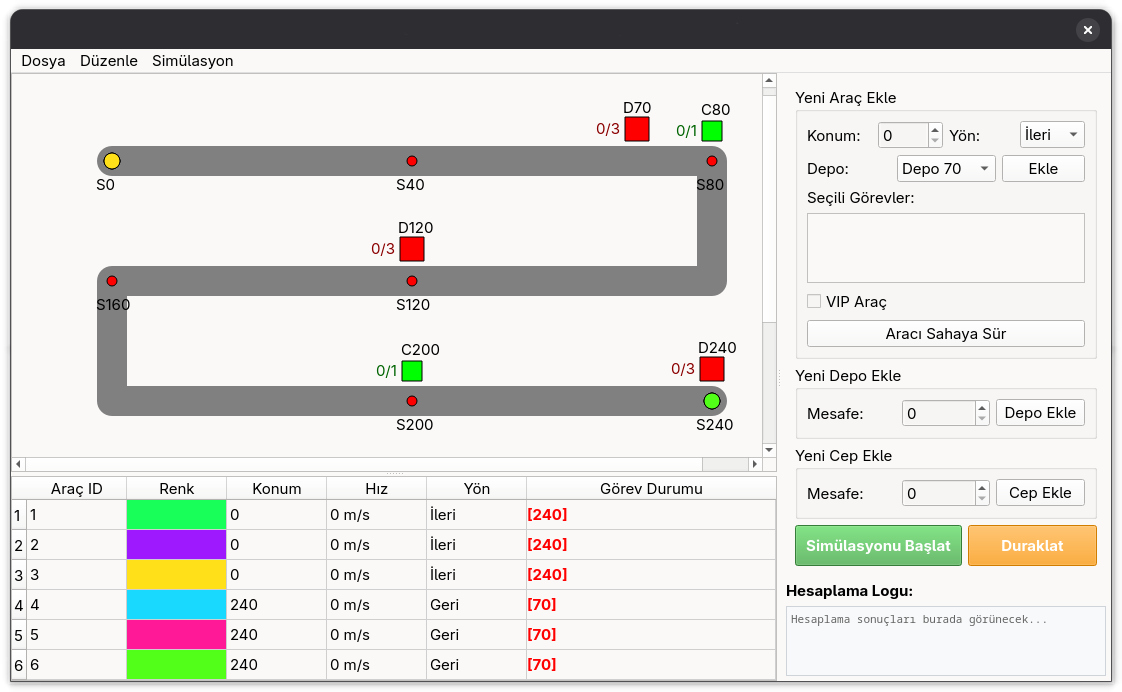
\includegraphics[width=0.7\linewidth]{img/senaryolar/0-zıt-yön-çatışması/00-başlangıç.png}
        \caption{\label{fig:zıt-yön-başlangıç}Zıt Yön Çatışması: Başlangıç Durumu}
    \end{figure}
 
    \subsubsection{Analiz}
    
    Başlangıç durumunda; (\autoref{fig:zıt-yön-başlangıç}) D240'da üç araç sola doğru yönde başlamaktadır, başlangıç konumunda ($x = 0$) ise üç araç sağ yönde başlamaktadır. Çizelgeleme algoritması gereği (\autoref{sec:önceliklendirme-ve-kilitlenme-çözümü}) önce D240'daki (A4, A5, A6) araçları önce çizelgelenmektedir. A5 ve A6 depoda beklerken A4 aracı D70'e doğru yola çıkmaktadır. Ardından güvenlik mesafesi korunarak A5 ve A6 araçları da D70 görevi için sırayla yola çıkıyorlar. Bu esnada başlangıç konumundaki A1, A2 ve A3 araçlarından A1 ve A2 yol vermek için D70 ve C80'de beklemektedirler (\autoref{fig:zıt-yön-araçların-beklemesi}).
    
    \begin{figure}[h!]
        \centering
        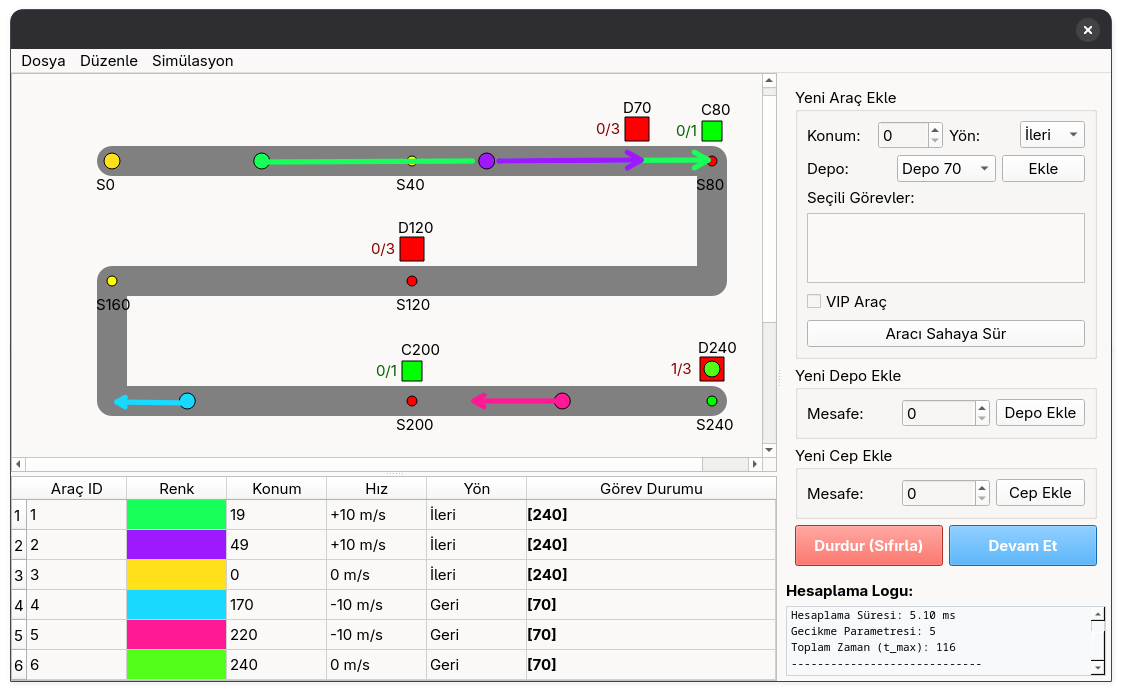
\includegraphics[width=0.7\linewidth]{img/senaryolar/0-zıt-yön-çatışması/01-ilk-iki-aracın-çıkışı (Edit).png}
        \caption{\label{fig:zıt-yön-ilk-iki-araç} İlk araçların çıkışı}
    \end{figure}
    
    A4, A5, A6 araçları D70 görevini tamamlayıp başlangıca döndükten sonra görevleri bitiyor. Ardından D70 ve C80'de bekleyen A1 ve A2 araçları sırayla D240 görevi için yola çıkmaktadırlar. Bu iki araçtan sonra A3 aracı en son yola çıkıp D120'de bu iki araca yol vermek için beklemektedir. Çizelgelemeye göre en başta olan A1 aracı yükünü alırken A2 aracı C200 cebinde bekleyip yol vermektedir. En son A3 aracı diğer araçlara yol verdikten sonra yükünü D240'dan alıp başlangıca döner (\autoref{fig:zıt-yön-son-araçların-yol-vermesi}).
    
    \begin{figure}[h]
        \centering
        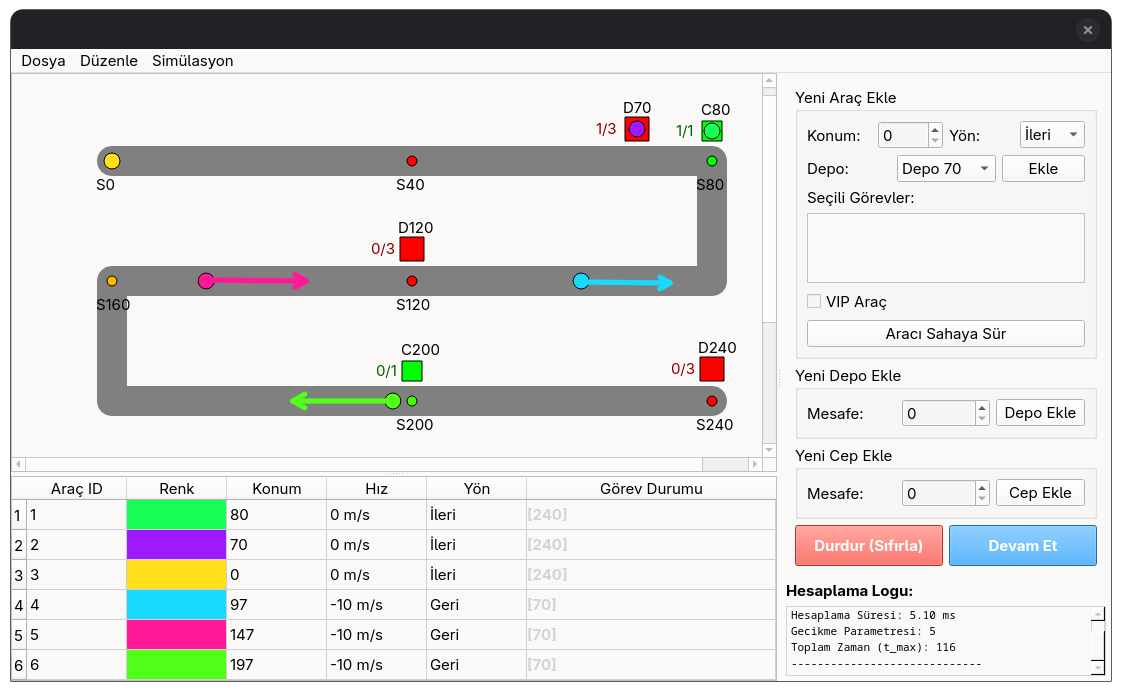
\includegraphics[width=0.7\linewidth]{img/senaryolar/0-zıt-yön-çatışması/02-araçların-beklemesi (Edit).png}
        \caption{\label{fig:zıt-yön-araçların-beklemesi} A1 ve A2 araçlarının beklemesi}
    \end{figure}
        
    \begin{figure}[h]
        \centering
        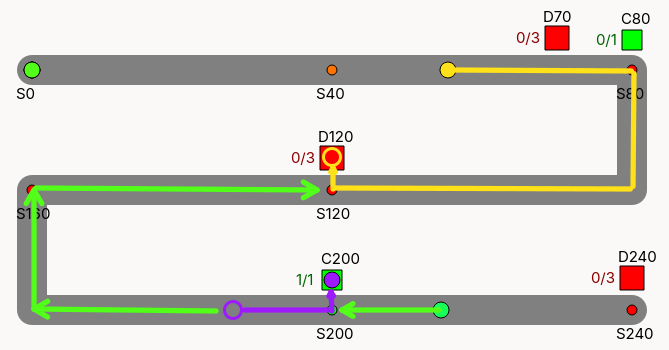
\includegraphics[width=0.7\linewidth]{img/senaryolar/0-zıt-yön-çatışması/03-son üç aracın birbirine yol vermesi (Edit).png}
        \caption{\label{fig:zıt-yön-son-araçların-yol-vermesi} A2 ve A3 aracının A1 aracına yol vermesi}
    \end{figure}
      
    \paragraph{Potansiyel Çarpışma Noktası} Kontrol mekanizması olmasaydı, zıt yönlü hareket eden $A_1$ ve $A_4$ araçları $t = 4$ anında $x = 120\text{ m}$ koordinatında kilitlenme (\textit{deadlock}) veya kafa kafaya çarpışma yaşayacaktı.
    
    \paragraph{Kilitlenme Analizi} $A_1$ aracı $C_{80}$ cebine çekilerek bekletilmiş, böylece kilitlenme olasılığı matematiksel kısıtlara uygun olarak sıfıra indirilmiştir.
    
    \subsubsection{Sonuç}
    
    Yapılan analiz sonucunda çizelgelemeye uygun olarak hareketlerine başlayan araçlar cepler ve depoları kullanarak birbirlerine yol vererek sırayla görevlerini tamamladıkları görülmüştür. Algoritmanın hesaplama süresi ve toplam zaman adımı (\textit{makespan}) \autoref{tab:zıt-yön-tablo}'da gösterilmiştir.
    
    \begin{table}[h]
        \centering
        \caption{Sonuçlar} \label{tab:zıt-yön-tablo}
        \begin{tabular}{lr}
            \hline
            Hesaplama Süresi (ms) & 5.10 \\
            \hline
            Toplam Zaman Adımı ($t_{max}$) & 116 \\
            \hline
        \end{tabular}
    \end{table}

\subsection{Darboğaz Sınaması} \label{sec:darboğaz-sınaması}
  
    Bu senaryoda araçların hepsinin tek bir depoya yoğunlaştığı durumda düzeneğin nasıl davrandığı incelenecektir. Amaca uygun olarak 10 tane araç başlangıç konumunda ve hepsinin görevi sadece D70 olacak biçimde yapılandırma yapılmıştır. Ardından sistem optimizasyonu üzerine etkisini gözlemlemek için araçların kullanabileceği bir cep sisteme eklenerek aynı senaryo tekrarlanmıştır.
    
    \subsubsection{Yapılandırma}
    
        Araçlar $t = 0$ anında aşağıdaki konumlarda başlamaktadırlar. $A = \{1, 2, 3, 4, 5, 6, 7, 8, 9, 10 \}$ araçları için $X_{t = 0}$-konum vektörü olmak üzere:
    
    \begin{equation}
        X_{t = 0} = \{0, 0, \dots, 0 \}
    \end{equation}
    
    \begin{itemize}
        \item $\text{Görevler} = \{\{70\}, \dots, \{70\}\}$
        \item $\text{Yönler} = \{ 1, \dots, 1\}$
        \item $G = \{ 70\}$
        \item $C = \emptyset $
    \end{itemize}
    
    \subsubsection{Analiz}
    
    Araçlar çizelgeleme mantığına uygun olarak kimlik numaralarına göre sırayla başlangıçtan hareket edip D70 deposuna gitmektedirler (\autoref{fig:darboğaz-başlangıç}). Bir araç yoldayken başka bir araç depoya hareket etmemektedir (\autoref{fig:darboğaz-cepsiz}). Arada bir cep olmadığından ve araçlar depoda yeteri kadar süre beklemediğinden darboğaz oluşmaktadır.
    
    \begin{figure}[h]
        \centering
        
\includegraphics[width=0.7\linewidth]{img/senaryolar/1-darboğaz/00-başlangıç.png}
        \caption{\label{fig:darboğaz-başlangıç} Darboğaz Sınaması: Başlangıç Durumu}
    \end{figure}

    Bu durumu çözmek için araya bir cep eklenebilir (\autoref{fig:darboğaz-cepli}). Cepler kümesi $C = \{ 30 \} $ olacak biçimde güncellenerek \autoref{fig:darboğaz-cepli}'deki yol yapılandırması elde edilmiştir. Cep eklendiği durumda iki araç peş peşe (güvenlik mesafesini koruyarak) çıkacaklar ve öndeki araç depodan dönüp aradaki cebi geçtikten sonra diğer cepteki araç depoya gidecektir. Cep boşaldıktan sonra ise üçüncü araç cebe girecektir. Bu durumu peş peşe çizelgelenen her araç için tekrarlanır. 
    
    Ceplerin eklenmesi durumunda araçlar hedeflerine daha yakın bir mesafeden başlayacaktır. Beklendiği üzere toplam zaman adımı ($t_{max}$) 171'den 135'e düşmüştür.
    
    \begin{figure}[h]
        \begin{subfigure}{.5\textwidth}
            \centering
            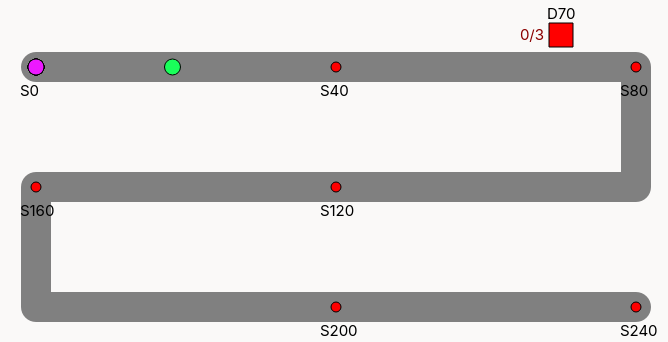
\includegraphics[width=0.9\linewidth]{img/senaryolar/1-darboğaz/01-ilk-araç.png}
            \caption{Cepsiz Durum $t_{max} = 171$}
            \label{fig:darboğaz-cepsiz}
        \end{subfigure}%
        \begin{subfigure}{.5\textwidth}
            \centering
            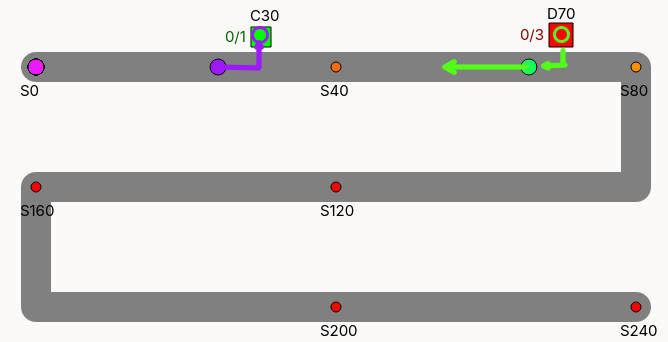
\includegraphics[width=0.9\linewidth]{img/senaryolar/1-darboğaz/02-cep-olma-durumu (Edit).png}
            \caption{Cepli Durum $t_{max} = 135$}
            \label{fig:darboğaz-cepli}
        \end{subfigure}
        \caption{Cepli ve Cepsiz Durumlarda Hareket Yönleri}
        \label{fig:darboğaz-cepli-cepsi}
    \end{figure}
    
    \subsubsection{Sonuç}

    Yapılan analiz sonucu açıkça görüldüğü üzere algoritma 10 aracın darboğaz oluşturduğu senaryoda tüm araçları başarıyla çizelgelemiş ve çarpışma durumu olmadan her aracın görevini tamamladığı gözlemlenmiştir. Darboğaz senaryosu depo ile başlangıç arasına bir cep eklenerek tekrarlandığında ise toplam zaman adımının azaldığı, hesaplama süresinin düştüğü ve araçların cepleri etkin biçimde kullanarak sistem optimizasyonunu artırdığı gözlemlenmiştir (\autoref{tab:darboğaz-tablo}).
    
    \begin{table}[h]
        \centering
        \caption{Sonuçlar} \label{tab:darboğaz-tablo}
        \begin{tabular}{l|l|l}
            Senaryo & Hesaplama Süresi [ms] & Toplam Zaman Adımı ($t_{max}$) \\
            \hline
            Cepsiz & 6.58  & 171 \\
            \hline
            Cepli & 4.43  & 135 \\
        \end{tabular}
    \end{table}

    \subsection{Stres Sınaması}\label{sec:stres-sınaması}
    
    Bu senaryoda sisteme görevleri değişen ve keyfi olarak atanmış, başlangıç noktasında konumlanan 21 araç verilmiştir (\autoref{fig:stres-görev-tablosu}). Sistemin fazla araç durumunda davranışı incelencektir. Senaryo, ceplerin ve depoların kullanımı sonucu zaman adımı değişimini ölçmek adına 21 tane sadece D240 görevine sahip araç ile tekrarlanmıştır.
        
    \begin{figure}[h]
        \centering
        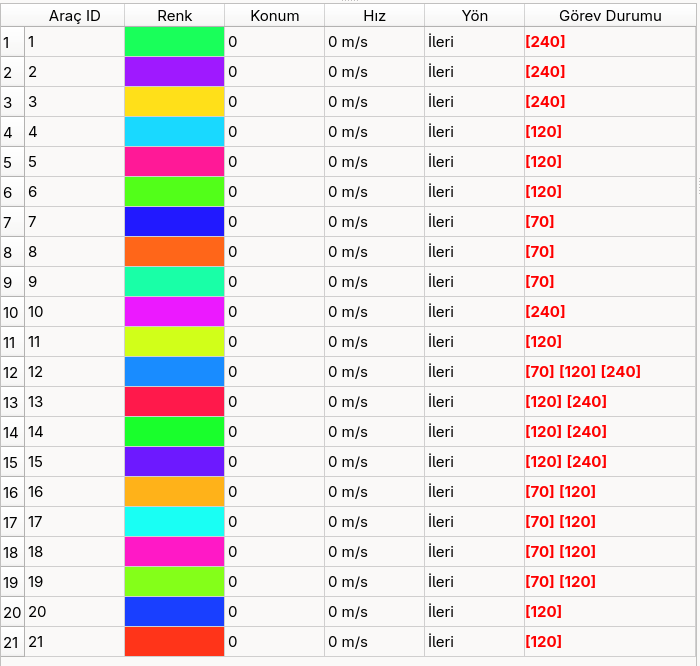
\includegraphics[width=0.7\linewidth]{img/senaryolar/2-stres/00-görev-tablosu.png}
        \caption{21 Araçlık Görev Tablosu}
        \label{fig:stres-görev-tablosu}
    \end{figure}
    
    \subsubsection{Analiz}
    
    $t_{max} = 526$ adımda ve 50.30 ms hesaplama süresiyle tüm araçlar çarpışma ve kilitlenme durumu olmadan görevlerini tamamlamıştır. Araçların görevleri boyunca cepleri ve depoları birbirlerine yol vermek için kullandıkları görülmüştür (\autoref{fig:stres-görev-anlık-görüntü}). Araçların ceplerde veya depolarda beklerken gereksiz girme çıkma durumları yerine daima bekledikleri gözlemlenmiştir.
    
    Araçların sadece D240 görevine sahip olduğu senaryodaysa (\autoref{fig:stres-tek-görev-başlangıç}) araçlar peş peşe başlangıçtan çıkmış ve sırayla uygun depo ve ceplerde önlerindeki aracın dönüşüne yol vermek için beklemeye geçmişlerdir.
    
    \begin{figure}[h]
        \begin{subfigure}{.5\textwidth}
            \centering
            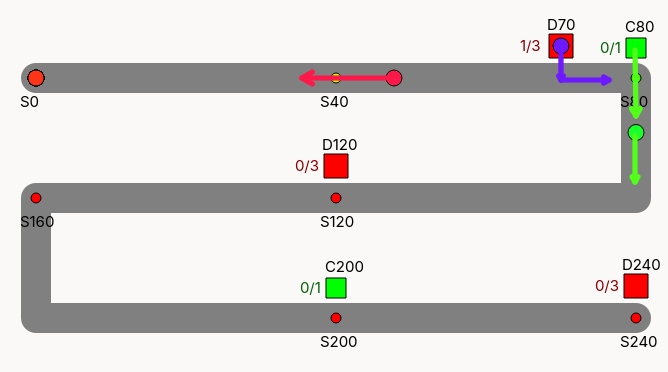
\includegraphics[width=0.9\linewidth]{img/senaryolar/2-stres/01-rastgele-bir-anda (Edit).png}
            \caption{Keyfi Görevler}
            \label{fig:stres-rastgele-bir-an}
        \end{subfigure}
        \begin{subfigure}{.5\textwidth}
            \centering
            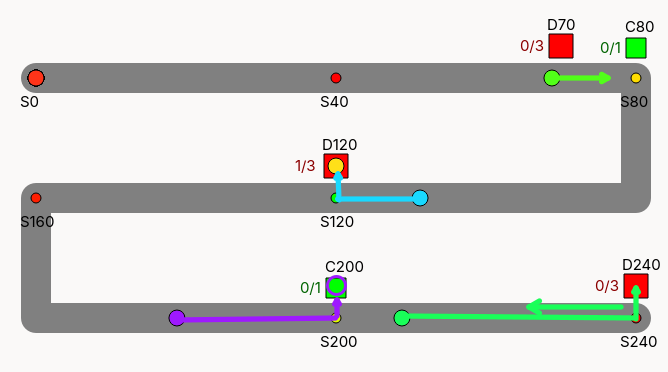
\includegraphics[width=0.9\linewidth]{img/senaryolar/2-stres/02-tek-görev-başlangıç (Edit).png}
            \caption{Tek Görev Durumu}
            \label{fig:stres-tek-görev-başlangıç}
        \end{subfigure}
        \caption{Görev Tablosu ve Sistemin Anlık Görüntüsü}
        \label{fig:stres-görev-anlık-görüntü}
    \end{figure}
    
    \subsubsection{Sonuçlar}
    
    21 araçlık senaryodaki hesaplamalar sistemde herhangi bir takılmaya neden olmadan kısa bir sürede tamamnlamıştır. Peş peşe birçok aracın \autoref{sec:darboğaz-sınaması}'de olduğu gibi aynı depoya gitmelerinden ötürü oluşan darboğaz gibi nedenlerden dolayı zaman adımının epey fazla olduğu gözlemlenmiştir.
    
    Tek görevin olduğu senaryo ile kıyaslandığında (\autoref{tab:stres-tablo}) hesaplama süresinin neredeyse 3 katına çıktığı toplam zaman adımının da 54-adım kadar düştüğü gözlemlendi. Zaman araçların başlangıçta zaman kaybetmek yerine depoda beklemesi sonucu azalsa da her t-anında yolda birçok aracın sürekli karşılaşmasından ötürü hesaplama süresi artmıştır.
    
    
    \begin{table}[h]
        \centering
        \caption{Sonuçlar} \label{tab:stres-tablo}
        \begin{tabular}{l|l|l}
            Görevler & Hesaplama Süresi [ms] & Toplam Zaman Adımı ($t_{max}$) \\
            \hline
            Değişen & 50.3  & 526 \\
            \hline
            Tek & 146.32  & 472 \\
        \end{tabular}
    \end{table}
    
    \subsection{Özel Öncelikli Araç}
    
    Bu bölümde özel öncelikli olarak belirlenen araçlara diğer araçların yol vermesi incelenecektir.
    
    \subsubsection{Yapılandırma}
    
        Araçlar $t = 0$ anında aşağıdaki konumlarda başlamaktadırlar. $A = \{1, 2, 3, 4, 5\}$ araçları için $X_{t = 0}$-konum vektörü olmak üzere:
    
    \begin{equation}
        X_{t = 0} = \{0, 0, 0, 30, 0 \}
    \end{equation}
    
    A1, A2 ve A3 araçları özel öncelikli (\textit{VIP}) araçlar olmaktadırlar. Her araç daima bu araçlara yol önceliği tanımaktadır.
    
    \begin{itemize}
        \item $\text{Görevler} = \{ \{240\}, \{120\}, \{70\}, \{70\}, \{70\} \}$
        \item $\text{Yönler} = \{ 1, 1, 1, 1, 1 \}$
        \item $G = \{ 70, 120, 240 \}$
        \item $C = \{ 80, 200 \}$
    \end{itemize}
    
    \begin{figure}[h]
        \centering
        
\includegraphics[width=0.7\linewidth]{img/senaryolar/4-vip-araç/00-başlangıç.png}
        \caption{Önceliki Araçlar: Başlangıç Durumu}
        \label{fig:vip-başlangıç}
    \end{figure}
    
    A4 aracı $(x=30, t=0)$ konumundan başlatılarak bu aracın öncelikli araçlardan önde yer alması ve öncelikli araçlara yol verme davranışının incelenmesi amaçlanmıştır. (\autoref{fig:vip-başlangıç})
    
    \subsubsection{Analiz}
    
    Başlangıçta A4 aracı D70 deposuna girdikten sonra A1, A2 ve A3 araçları $x = 70$ konumunu geçip geri dönüş yolunu boşaltana kadar depoda beklemeye devam etmektedir. Başka bir ifadeyle A4 aracı öncelikli araçlar yolu boşaltana kadar yol hakkın kendisinde olmasına rağmen depoda beklemeye devam etmektedir.
        
    \begin{figure}[h]
        \begin{subfigure}{.5\textwidth}
            \centering
            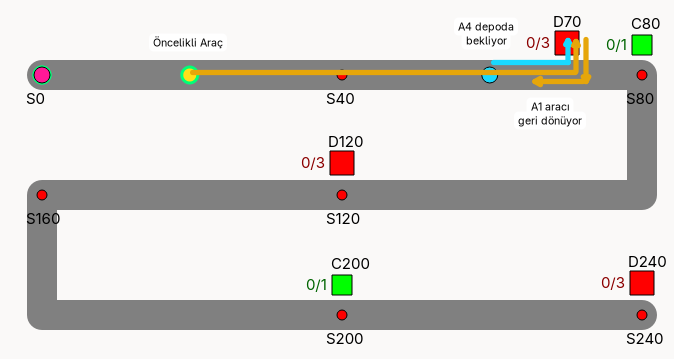
\includegraphics[width=0.9\linewidth]{img/senaryolar/4-vip-araç/01-vip-araca-yol-verme (Edit).png}
            \caption{A4 Aracı Öncelikli A1 Aracına Yol Veriyor}
            \label{fig:vip-yol-verme-0}
        \end{subfigure}
        \begin{subfigure}{.5\textwidth}
            \centering
            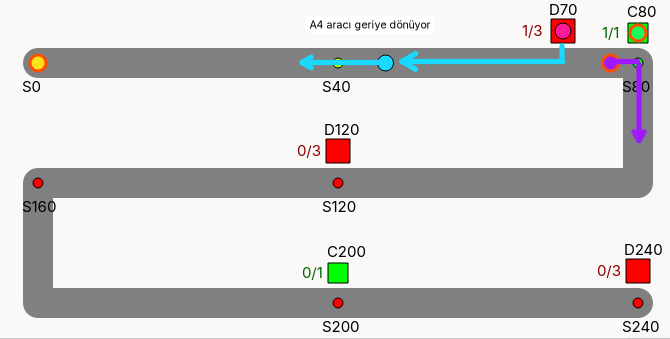
\includegraphics[width=0.9\linewidth]{img/senaryolar/4-vip-araç/02-düşük-öncelikli-en-son geri dönüyor (Edit).png}
            \caption{A4 Aracının Geri Dönüşü}
            \label{fig:vip-en-son-geri-dönme}
        \end{subfigure}
        \caption{Öncelikli Araçlara Yol Verilmesi}
        \label{fig:vip-yol-verme}
    \end{figure}
    
    \subsection{Dinamik Başlangıç}
    
    Bu senaryoda başlangıç dışında yolun ortasında başlayan araçlar ve tek bir depo kullanılarak algoritmanın dinamik başlangıçlarda kilitlenmeyi nasıl çözdüğü incelenecektir.
    
    \subsubsection{Yapılandırma}
    
    Araçlar $t = 0$ anında aşağıdaki konumlarda başlamaktadırlar. $A = \{1, 2, 3, 4, 5, 6, 7, 8, 9, 10, 11\}$ araçları için $X_{t = 0}$-konum vektörü olmak üzere:
    
    \begin{equation}
        X_{t = 0} = \{0, 0, 0, 0, 200, 240, 160, 80, 40, 60, 120 \}
    \end{equation}
    
    \begin{itemize}
        \item $\text{Görevler} = \{ \{120\}, \dots \}$
        \item $\text{Yönler} = \{ 1, 1, 1, 1, -1, \dots -1 \}$
        \item $G = \{ 120 \}$
        \item $C = \{ 60, 220 \}$
    \end{itemize}
    
    \begin{figure}[h]
        \centering
        
\includegraphics[width=0.7\linewidth]{img/senaryolar/5-dinamik-başlangıç/00-başlangıç.png}
        \caption{Dinamik Başlangıç Durumu}
        \label{fig:dinamik-başlangıç}
    \end{figure}
    
    \subsubsection{Analiz}
    
    \autoref{sec:önceliklendirme-ve-kilitlenme-çözümü}'de bahsedilen çizelgelemeye göre, önce çizelgelenen araç hedefine en yakın olan $x = 120$ konumunda başlayan A11 aracıdır. Bu aracın bulunduğu konumdaki depoya girdikten sonra doğrudan başlangıç konumuna yönelmektedir. Bu sırada yolundaki araçlardan A10 aracı bulunduğu konumdaki cebe girerken A8 ve A9 araçları ise yol verecek bir yer olmamasından ötürü başlangıç konumuna gitmektedir.
     
     \paragraph{Ceplerin Kaldırılması} C60 ve C220 ceplerinin kaldırılması durumunda ise program güvenli mesafe kuralının sağlanamaması durumundan ve rota bulunamamasından ötürü kilitlenme uyarısı vermektedir \autoref{fig:dinamik-kilitlenme-hata}.
    
    \begin{figure}[h]
        \centering
        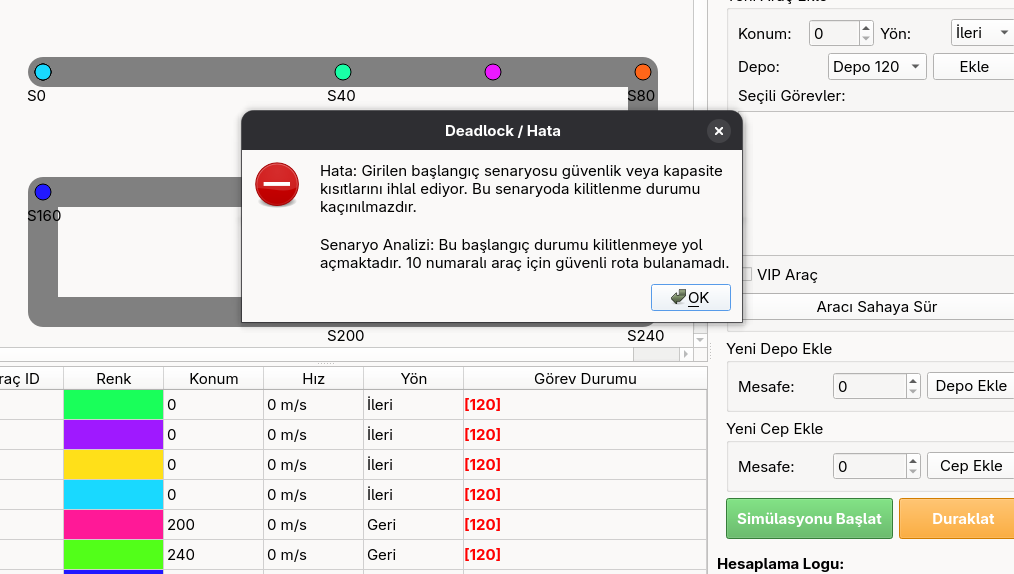
\includegraphics[width=0.7\linewidth]{img/senaryolar/5-dinamik-başlangıç/01-kilitlenme-uyarısı.png}
        \caption{Kilitlenme Uyarısı}
        \label{fig:dinamik-kilitlenme-hata}
    \end{figure}
    
    \subsection{Performans Analizi}
    
    Analizi yapılan senaryolar ardından sistem \autoref{sec:stres-sınaması}'daki tek görevli senaryo baz alınarak farklı araç sayılarındaki hesaplama performansı test edilmiştir.
    
    \begin{table}[!ht]
        \centering
        \caption{Sonuçlar} \label{tab:performans-tablo}
        \begin{tabular}{l|l|l}
            Araç Sayısı & Hesaplama Süresi (ms) & Toplam Zaman \\ \hline
            5 & 11.1 & 136 \\ \hline
            11 & 43.37 & 262 \\ \hline
            14 & 68.0 & 317 \\ \hline
            21 & 146.32 & 472 \\ \hline
            30 & 297.04 & 653 \\ \hline
            33 & 518.83 & 724 \\ \hline
            36 & 1291.78 & 779 \\ \hline
            39 & 2490.93 & 850 \\ \hline
            42 & 3854.37 & 905 \\
        \end{tabular}
    \end{table}
    
    \autoref{fig:performans-hesaplama}'de gözüktüğü üzere hesaplama zamanı araç sayısı arttıkça üstel olarak artmaktadır. Toplam görev tamamlanma zamanıysa (\autoref{fig:performans-zaman}) araç sayısına bağlı olarak doğrusal bir artış eğilimindedir.
    
    \begin{figure}[h]
        \centering
        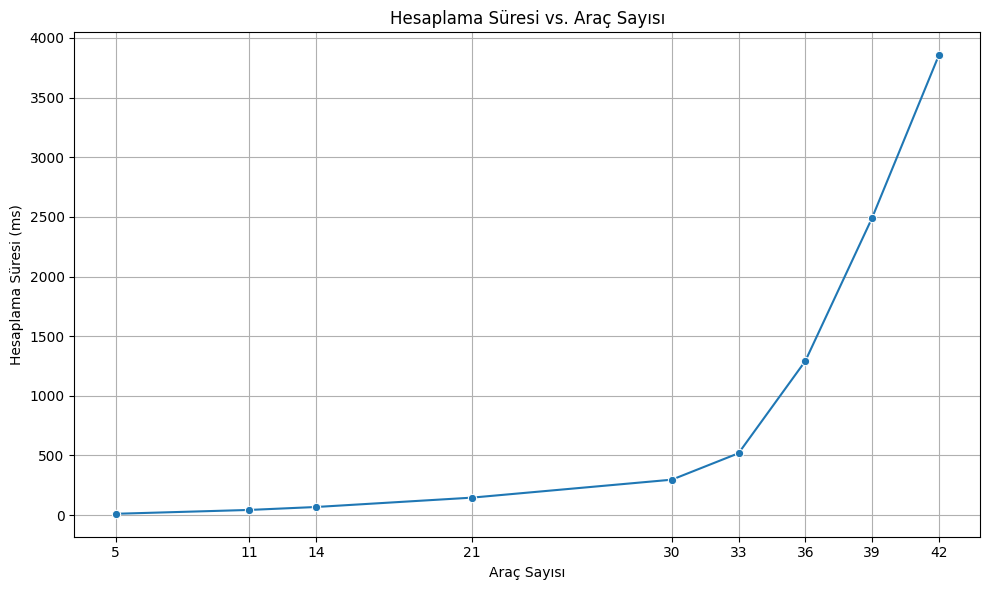
\includegraphics[width=0.9\linewidth]{img/senaryolar/3-performans/hesaplama-süresi-grafik.png}
        \caption{Hesaplama Süresi - Araç Sayısı}
        \label{fig:performans-hesaplama}
    \end{figure}
    
    \begin{figure}[h]
        \centering
        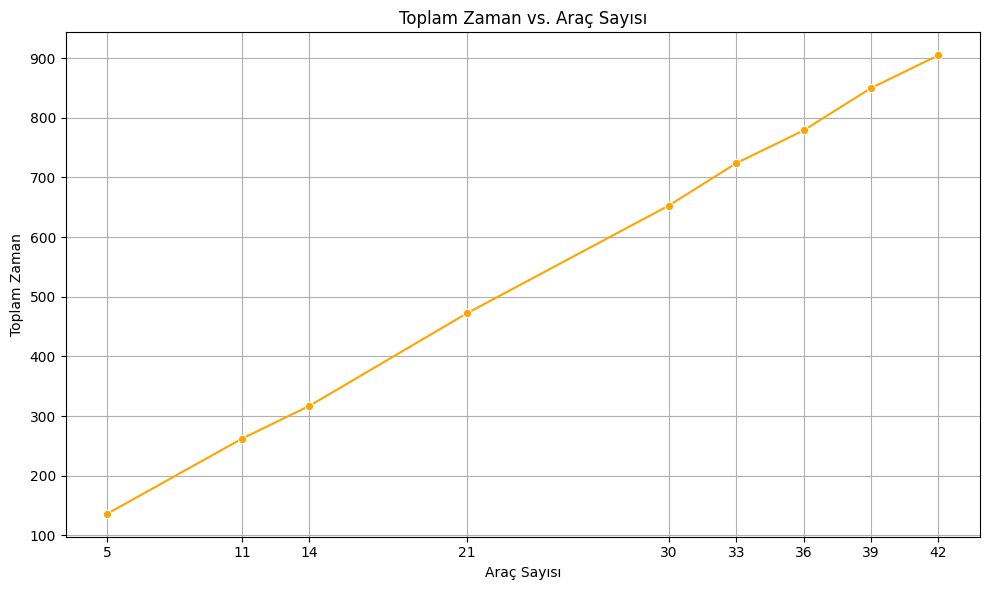
\includegraphics[width=0.9\linewidth]{img/senaryolar/3-performans/zaman-adımı-grafik.png}
        \caption{Toplam Zaman - Araç Sayısı}
        \label{fig:performans-zaman}
    \end{figure}
